\documentclass[language=polish,type=eng]{aghmodern}

\titleEN{Capture-The-Flag game based on reverse engineering}
\titlePL{Gra typu Capture-The-Flag oparta o reverse engineering}
\author{Piotr Szczygieł}
\faculty{Wydział Informatyki, Elektroniki i Telekomunikacji}
\department{Katedra Informatyki}
\supervisor{dr inż. Łukasz Faber}
\degreeprogramme{Informatyka}
\degreetype{Stacjonarne}
\date{2020}

\usepackage[backend=biber,doi=true,url=false]{biblatex}
\addbibresource{bibliography.bib}

\usepackage{minted}
\usepackage{perpage}
\MakePerPage{footnote}

\graphicspath{ {./images/} }

\begin{document}

\frontmatter
\maketitle
\tableofcontents

\mainmatter

\chapter{Cel prac i wizja produktu}

\section{Wprowadzenie}

Gra typu Capture-the-Flag jest to rodzaj zawodów z ogólnie pojętego
bezpieczeństwa komputerowego. Ich celem zwykle jest edukacja uczestników
o zabezpieczeniach systemów oraz możliwość pokazania im jak reagować
na wypadek wystąpienia rzeczywistych ataków. Zawody takie podzielone są zazwyczaj
na poszczególne zadania z różnych kategorii. Aby rozwiązać takie zadanie należy
znaleźć ,,flagę'', którą następnie podaje się w interfejsie udostępnionym przez
organizatora zawodów. Flagą w tym wypadku jest ciąg znaków, który możemy uzyskać
poprzez rozwiązanie zadania. Przykładowo w najprostszych zadaniach
z dziedziny eksploitacji stron internetowych, flagę możemy znaleźć klikając
,,Pokaż źródło strony'' w przeglądarce internetowej.

\begin{figure}[H]
\centering
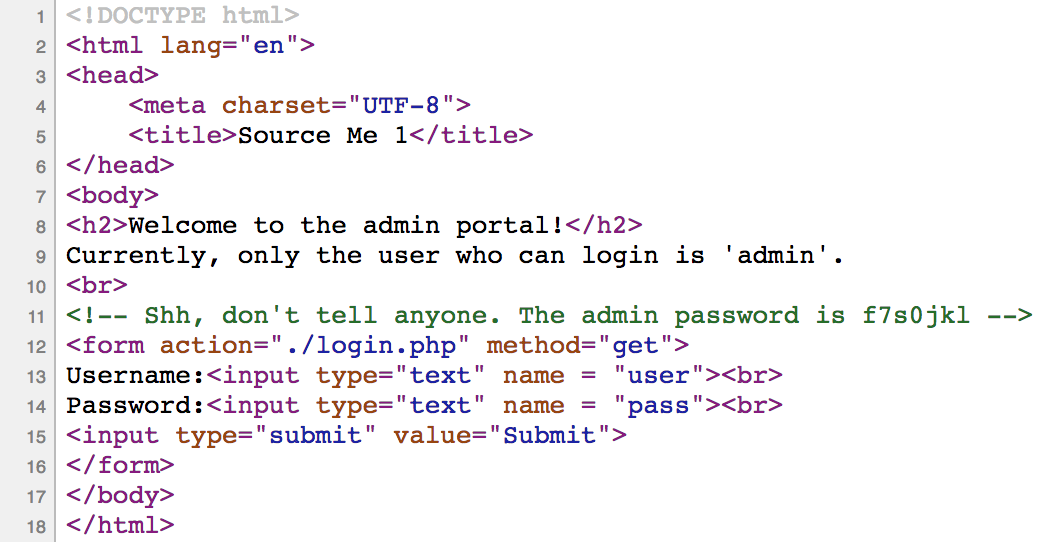
\includegraphics[width=10cm]{flag_page_source}
\caption{Flaga \emph{f7s0jkl} ukryta w źródle strony internetowej}
\end{figure}

W tej pracy zaprezentowana będzie jednak grę oparta
wyłącznie o Reverse Engineering (ang. Inżynieria Wsteczna).
Inżynieria wsteczna oprogramowania może odbywać się na różne sposoby.
Może to być przykładowo wykorzystanie tzw. snifferów do analizy protokołów
komunikacyjnych aplikacji internetowej. W tym wypadku będzie ona jednak
zazwyczaj oznaczała proces analizy programu, aby zrozumieć co robi
oraz w jaki sposób. Przedstawione zadania można by też podpiąć do kategorii
eksploitacji binarnej (ang. Binary Exploitation), która w pewny sposób pokrywa
się z zagadnieniami Reverse Engineeringu. Jest to mianowicie proces
wykorzystywania niedoskonałości programów w celu zmuszenia ich do zrobienia
czegoś, czego w normalnej sytuacji nie powinny robić. Te dwie kategorie pokrywają
się ze sobą, ponieważ zazwyczaj nie jest możliwe rozwiązanie zadania z kategorii
eksploitacji binarnej, bez wykorzystania do tego inżynierii wstecznej.

Produktem końcowym będzie zbiór kilku zadań udostępniony na platformie webowej.
Platforma sama w sobie nie jest niczym specjalnym, udostępnia jedynie takie powszechne
funkcjonalności jak rejestracja użytkowników, ranking najlepszych graczy,
pobieranie zadań oraz interfejs umożliwiający wprowadzanie znalezionych
flag. Z tego względu użyta zostanie gotowa platforma CTFd\footnote{\url{https://ctfd.io/}}.
Użycie takiego gotowego rozwiązania pozwoli w pełni skupić się na samych zadaniach,
a ominąć takie kwestie jak np. gracze łamiący zabezpieczenia platformy.

\begin{figure}[H]
\centering
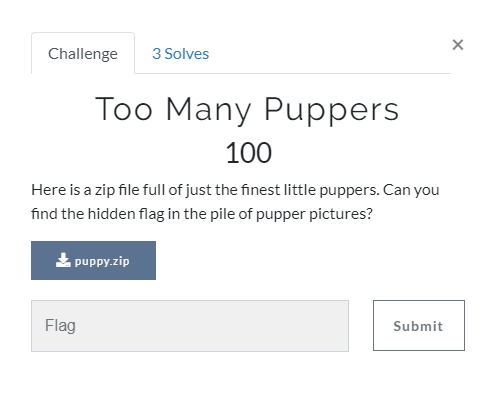
\includegraphics[width=10cm]{ctfd}
\caption{Przykładowe zadanie na stronie demonstracyjnej CTFd}
\end{figure}

W tej pracy opisany zostanie zarówno proces tworzenia poszczególnych zadań,
jak i przykładowe ich rozwiązania. Użyte zostało słowo "przykładowe", ponieważ
w takiej kategorii jak Binary Exploitation / Reverse Engineering liczba sposobów
na rozwiązanie danego zadania jest ograniczona jedynie przez wyobraźnie uczestnika.
Nie ograniczymy się również do korzystania ciągle z tych samych narzędzi.
Pokazane zostaną różnorodne podejścia do analizy i rozwiązywania wyzwań.
Zadania będą tworzone z zamiarem zachowania rosnącego stopnia trudności.
Na początku uczestnik będzie miał szansę rozwiązać proste zadania,
zachęcające go do dalszej rozgrywki. Finalne zadania powinny stanowić wyzwanie
nawet dla doświadczonych graczy.

\section{Dostępne platformy}

Aktualnie istnieje wiele różnych zawodów CTF online. Jednym z popularniejszych
jest \mbox{picoCTF}\footnote{\url{https://picoctf.com/}}.
Można tam wejść kiedykolwiek, zalogować się i zająć się rozwiązywaniem problemów.

\begin{figure}[H]
\centering
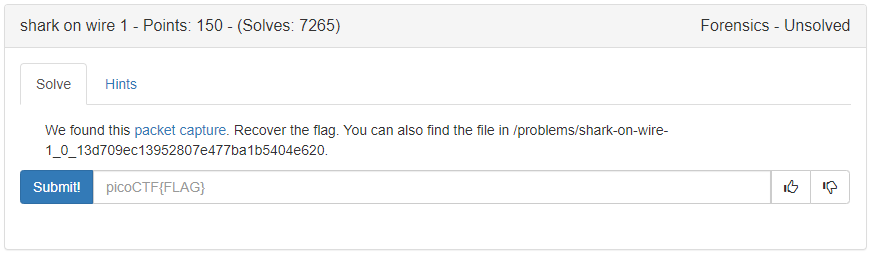
\includegraphics[width=\textwidth]{picoctf}
\caption{Zadanie z kategorii Forensics na stronie picoCTF}
\end{figure}

Główną motywacją do napisania tej pracy jest fakt, że strony tego typu często skupiają
się na zadaniach w takich kategoriach jak Forensics czy Web Exploitation.
Mnie natomiast bardzo interesuję temat inżynierii wstecznej i chciałem
przygotować wyzwania oparte o zadania tylko z tej kategorii.

\section{Języki programowania i narzędzia}

Zadania będą tworzone w języku C. Jest to powszechnie znany język, który
z wyłączoną zbyt agresywną optymalizacją ze strony kompilatora, generuje
w miarę przewidywalny kod maszynowy. Zaletą tego jest to, że narzędzia
do debugowania, deasemblacji oraz wykonywania innych analiz programów
dobrze radzą sobie z takimi plikami. Dzięki temu język ten
zapewni nam kontrolę nad tym w jakim stopniu graczowi ułatwimy
lub utrudnimy rozgrywkę. W celu zapewnienia większej różnorodności
środowisk korzystać będziemy zarówno z systemu Windows jak i Linux.

Do rozwiązywania zadań posłużymy się różnorodnymi rodzajami narzędzi.
Poczynając od linuksowych programów linii poleceń takich jak \mintinline{bash}{strings}
czy \mintinline{bash}{gdb}, pisania własnych narzędzi w języku \emph{Python},
czy w końcu korzystając z pełnoprawnych narzędzi z interfejsem graficznym takich
jak \emph{Cutter}, czy używana przez NSA \emph{Ghidra}.

\chapter{Zakres funkcjonalności}

\section{Platforma}

Do interfejsu webowego skorzystamy z gotowej platformy CTFd.
Finalny produkt będzie dostępny pod adresem
\href{https://ctf.szczygiel.dev}{https://ctf.szczygiel.dev}.
Strona postawiona będzie na prywatnym serwerze VPS. Platforma będzie
uruchomiona w środowisku docker, a wystawiona do świata będzie poprzez serwer
Caddy\footnote{\url{https://caddyserver.com/}}, który w prosty sposób zapewni nam HTTPS,
dzięki organizacji Let's Encrypt\footnote{\url{https://letsencrypt.org/}}.

\section{Użytkownicy}

Użytkownikiem systemu będzie każda osoba zainteresowana rozwiązywaniem
tego rodzaju zadań. Może to być zarówno ktoś kształcący się lub pracujący
w dziale informatycznym, jak i osoba dla której jest to jedynie hobby.

Wszystkie gotowe zadania zostaną wrzucone na platformę, dzięki czemu
każda zainteresowana osoba będzie mogła spróbować swoich sił.

\section{Zadania}

Każde z zadań będzie sprawdzało różne umiejętności rozwiązujących je użytkowników.
Kolejne zadania będą miały coraz większy stopień trudności. Liczba przy nazwie zadania
oznacza ilość punktów, które użytkownik dostanie za prawidłowe rozwiązanie.

\subsection{100-simple}
\subsection{200-game}
\subsection{300-strcmp}
\subsection{400-decrypt}
\subsection{500-secret-shell}
\subsection{600-vm}

\chapter{Wybrane aspekty realizacji}

\section{Wprowadzenie}

W tym rozdziale przedstawione zostaną sposoby tworzenia poszczególnych zadań.
Warto dodać również, że przestawione flagi są w formacie \emph{AGH\{nazwa-zadania\}},
aby nie wyjawiać prawdziwych flag użytych w rozgrywce.
Przykładowe rozwiązania zadań znajdują się w rozdziale 5 -- \nameref{chap:writeups}.

\section{Zadanie 100-simple}

Pierwszym zadaniem jest odnalezienie flagi wprost umieszczonej
w pliku wykonywalnym jako ciąg znaków.
Zadanie to służyć ma jako pewnego rodzaju rozgrzewka i powinno być stosunkowo
proste do rozwiązania nawet przez kompletnie początkujących zawodników.
Poniżej uproszczony\footnote{Uproszczony, czyli zawierający jedynie
najważniejsze fragmenty kodu, pozbawiony sprawdzania błędów, definicji funkcji
pomocniczych, załączania nagłówków itp.} kod programu.

\begin{minted}{c}
int main()
{
    char input[64];

    printf("Enter the flag: ");
    fgets(input, sizeof(input), stdin);

    input[strlen(input) - 1] = '\0';

    if (strcmp(input, "AGH{100-simple}") == 0) {
        puts("Correct flag!");
    } else {
        puts("Incorrect flag!");
    }

    return 0;
}
\end{minted}

Jak widać program jedynie co robi, to pobiera wejście od użytkownika, a następnie
porównuje je z zapisaną na stałe w kodzie flagą. Użytkownik po inspekcji skompilowanego
pliku wykonywalnego komendą \mintinline{bash}{strings} lub użyciu innego narzędzia
do inspekcji plików binarnych, powinien szybko zwrócić uwagę na
ciąg znaków wyglądający jak rozwiązanie tego zadania.

\section{Zadanie 200-game}

W drugim zadaniu flaga będzie odszyfrowana zaraz po uruchomieniu programu. Zadaniem
użytkownika będzie odnalezienie tej flagi poprzez modyfikacje
pliku wykonywalnego w celu zmiany zachowania programu.

Sam program będzie działać w graficznym środowisku systemu Windows.
Do obsługi okienek i innych aspektów graficznych wykorzystana została
biblioteka raylib\footnote{\url{https://www.raylib.com/}}.
Poniżej przedstawiony kod programu z pominięciem funkcji \emph{decrypt\_flag}.

\begin{minted}[breaklines]{c}
bool show_flag()
{
    return false;
}

int main()
{
    if (show_flag()) {
        decrypt_flag();
    }

    SetTraceLogLevel(LOG_ERROR);
    InitWindow(460, 40, "200-game");
    SetTargetFPS(60);

    while (!WindowShouldClose()) {
        BeginDrawing();
        ClearBackground(BLACK);

        if (show_flag()) {
            DrawText((const char*)flag, 10, 10, 20, GREEN);
        } else {
            DrawText("You have not unlocked access to the flag!", 10, 10, 20, RED);
        }

        EndDrawing();
    }

    CloseWindow();
    return 0;
}
\end{minted}

Sednem całego zadania jest funkcja \emph{show\_flag}, która kontroluje czy rozwiązanie
ukaże się użytkownikowi oraz czy flaga w ogóle zostanie odszyfrowana.
Jeśli chodzi o samo szyfrowanie flagi, użyte zostało do tego narzędzie\footnote{
zerosum0x0: Obfuscated String/Shellcode Generator - Online Tool
\url{https://zerosum0x0.blogspot.com/2017/08/obfuscatedencrypted-cc-online-string.html}}
pozwalające zamienić ciąg znaków na tablice bajtów wraz z algorytmem odszyfrowującym.
Poniżej przedstawiony fragment wyniku działania takiego narzędzia.

\begin{minted}{c}
unsigned char flag[] = {
    0xa6, 0x40, 0x70, 0x2b, 0x6e, 0xed, 0x80,
    0x19, 0x36, 0xe1, 0x8a, 0xcd, 0x98, 0xa2
};

void decrypt_flag()
{
    for (unsigned int m = 0; m < sizeof(flag); ++m) {
        unsigned char c = flag[m];
        c = (c >> 0x1) | (c << 0x7);
        c ^= 0x74;
        c = -c;
        c += 0x3f;

        ...

        c ^= 0xc8;
        c = ~c;
        c = -c;
        c -= 0x51;
        flag[m] = c;
    }
}
\end{minted}

Odszyfrowanie flagi korzystając z kodu zdekompilowanej funkcji \emph{decrypt\_flag} jest możliwe,
jednak użytkownik powinien sobie dużo szybciej poradzić z rozwiązaniem zadania prostszymi
sposobami.

\section{Zadanie 300-strcmp}

Trzecie zadanie będzie połączeniem dwóch wcześniejszych.
Poniżej przedstawiona funkcja \emph{main} programu.

\begin{minted}[breaklines]{c}
int main()
{
    decrypt_flag();

    char input[64];

    printf("Enter the flag: ");
    fgets(input, sizeof(input), stdin);

    input[strlen(input) - 1] = '\0';

    if (strcmp(input, (char*)flag) == 0) {
        puts("Correct flag!");
    } else {
        puts("Incorrect flag!");
    }

    return 0;
}
\end{minted}

Jak widać kod jest taki sam jak w zadaniu pierwszym, jedynie z tą różnicą, że
flaga zamiast zapisana w kodzie w jawny sposób, jest odszyfrowywana zaraz po uruchomieniu
programu -- podobnie jak w zadaniu drugim.

\section{Zadanie 400-decrypt}

Czwarte zadanie będzie zawierało funkcje szyfrującą wejście użytkownika, a następnie to wejście będzie
porównywane z wcześniej zaszyfrowaną flagą. Zadaniem użytkownika będzie przykładowo napisanie skryptu
odwracającego działanie funkcji szyfrującej i uruchomienie go podając na wejście zaszyfrowaną flagę
wyciągniętą z pliku wykonywalnego.

Funkcja szyfrującą będzie dzieliła się na dwa etapy. Pierwszym etapem będzie użycie prostego
szyfru Cezara z przesunięciem 13 -- zwanym także ROT13. Drugi etap będzie to prosty szyfr XOR
z użyciem 4 bajtowego klucza. Poniżej przestawiony kod funkcji \emph{main} programu.

\begin{minted}[breaklines]{c}
int main()
{
    char input[64];

    printf("Enter the flag: ");
    fgets(input, sizeof(input), stdin);

    int length = strlen(input) - 1;
    input[length] = '\0';

    if (length == sizeof(flag)) {
        encrypt(input, length);

        if (memcmp(input, flag, length) == 0) {
            puts("Correct flag!");
            return 0;
        }
    }

    puts("Incorrect flag!");
    return 0;
}
\end{minted}

Jak widać główny kod programu jest bardzo prosty i nie różni się specjalnie od poprzednich zadań.
Poniżej przedstawiona zostanie funkcja szyfrująca \emph{encrypt}.

\begin{minted}{c}
void encrypt(char* input, int length)
{
    for (int i = 0; i < length; ++i) {
        char c = input[i];

        if (c >= 'A' && c <= 'Z') {
            if (c + 13 <= 'Z')
                input[i] = c + 13;
            else
                input[i] = c - 13;
        } else if (c >= 'a' && c <= 'z') {
            if (c + 13 <= 'z')
                input[i] = c + 13;
            else
                input[i] = c - 13;
        }
    }

    char key[] = { 0xde, 0xad, 0xbe, 0xef };
    int k = 0;

    for (int i = 0; i < length; ++i) {
        input[i] ^= key[k];
        k = (k + 1) % sizeof(key);
    }
}
\end{minted}

Pierwsza część szyfrowania, czyli ROT13, przechodzi po kolei po każdym znaku na wejściu i jeśli jest to litera,
to przesuwa ją o 13 w lewo albo 13 w prawo. Druga część to prosty szyfr XOR z kluczem \emph{0xde, 0xad, 0xbe, 0xef}.
Program przechodzi po kolei po każdym znaku i wykonuje operacje XOR z kolejnymi bajtami klucza. Jeśli dojdziemy
do ostatniego bajta klucza -- wracamy z powrotem do pierwszego bajtu.

Ostatnim krokiem jest wygenerowanie tablicy \emph{flag}. Tworzymy nowy pomocniczy program
-- \emph{generate}, zawierający zmodyfikowaną funkcję \emph{main},
która zwróci nam finalną zawartość tablicy \emph{flag}.
Poniżej przestawiony zmodyfikowany kod funkcji \emph{main} dla programu \emph{generate}.

\begin{minted}{c}
int main()
{
    char input[64];
    fgets(input, sizeof(input), stdin);

    int length = strlen(input) - 1;
    input[length] = '\0';

    encrypt(input, length);

    for (int i = 0; i < length; ++i) {
        printf("0x%02x, ", (unsigned char)input[i]);
    }

    return 0;
}
\end{minted}

Kompilujemy i uruchamiamy program, podając mu na wejście flagę, którą użytkownik będzie musiał odgadnąć.

\begin{minted}[breaklines]{text}
$ make generate
gcc -Wall -Wextra -std=c99 generate.c -o generate
$ ./generate
AGH{400-decrypt}
0x90, 0xf9, 0xeb, 0x94, 0xea, 0x9d, 0x8e, 0xc2, 0xaf, 0xdf, 0xce, 0x8a, 0xb2, 0xce, 0xd9, 0x92,
\end{minted}

Teraz możemy do głównego programu dodać definicje tablicy \emph{flag}.

\begin{minted}[breaklines]{c}
char flag[] = { 0x90, 0xf9, 0xeb, 0x94, 0xea, 0x9d, 0x8e, 0xc2, 0xaf, 0xdf, 0xce, 0x8a, 0xb2, 0xce, 0xd9, 0x92 };
\end{minted}

\section{Zadanie 500-secret-shell}

\section{Zadanie 600-vm}

\chapter{Organizacja pracy}

\chapter{Przykłady rozwiązań zadań}
\label{chap:writeups}

\section{Wprowadzenie}

W tym rozdziale przedstawione zostaną przykładowe sposoby rozwiązania poszczególnych zadań.
Podobnie jak w rozdziale opisującym proces tworzenia tych zadań, znalezione
flagi są przykładowe.

Aby rozpocząć rozwiązywać zadania użytkownik musi się udać na stronę z zadaniami.

\begin{figure}[H]
\centering
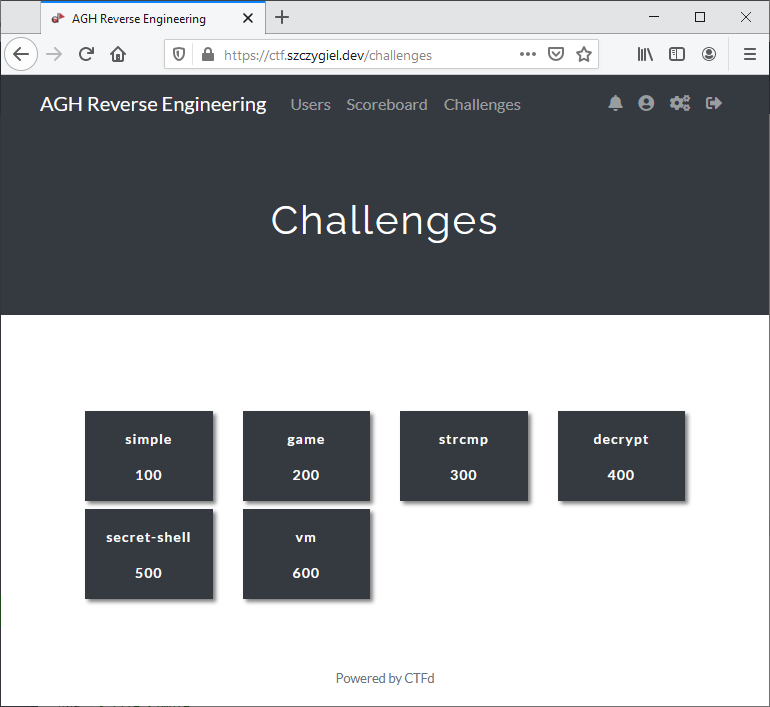
\includegraphics[width=\textwidth]{ui_challenges}
\caption{Interfejs użytkownika z listą zadań do rozwiązania}
\end{figure}

Po wybraniu zadania do rozwiązania ukazuję mu się okno,
gdzie może pobrać plik z zadaniem oraz wprowadzić rozwiązanie.

\begin{figure}[H]
\centering
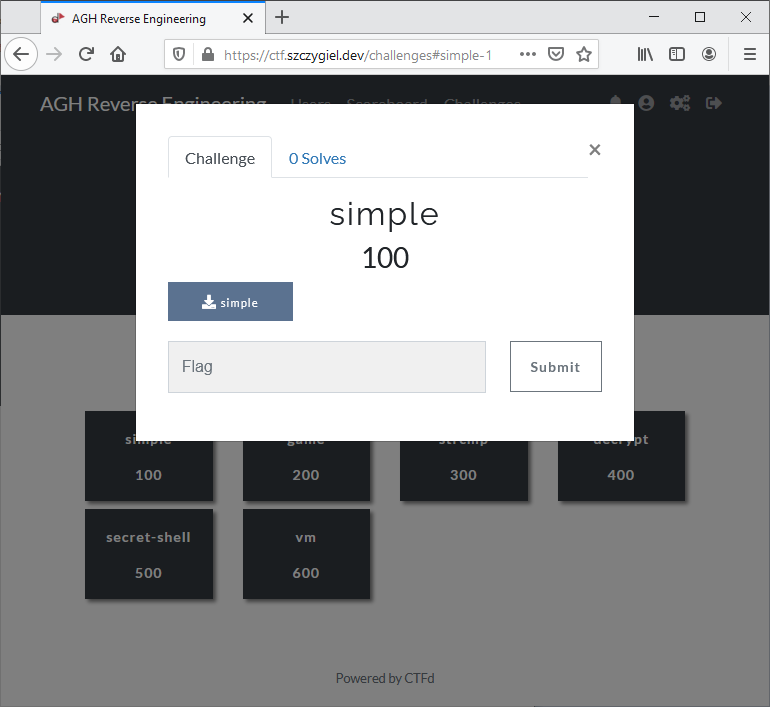
\includegraphics[width=\textwidth]{ui_download}
\caption{Interfejs użytkownika z konkretnym zadaniem do rozwiązania}
\end{figure}

\begin{figure}[H]
\centering
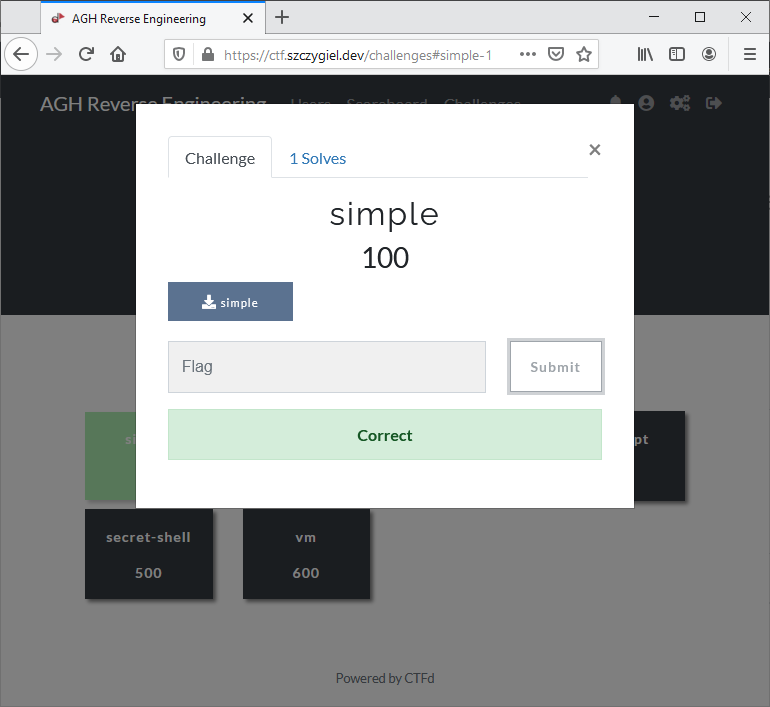
\includegraphics[width=\textwidth]{ui_solved}
\caption{Interfejs użytkownika po wprowadzeniu prawidłowej flagi}
\end{figure}

\section{Zadanie 100-simple}

Po otworzeniu karty z pierwszym zadaniem uczestnik pobiera załączony do niego
plik -- \emph{simple}.
Na początku sprawdza z jakim rodzajem pliku ma do czynienia.

\begin{minted}[breaklines]{text}
$ file simple
simple: ELF 64-bit LSB pie executable, x86-64, version 1 (SYSV), dynamically linked, interpreter /lib64/ld-linux-x86-64.so.2, BuildID[sha1]=4bfaf13eb10701fb33b5442a8e17056253509ef1, for GNU/Linux 3.2.0, with debug_info, not stripped
\end{minted}

Jak zauważa, jest to plik wykonywalny dla 64-bitowego systemu Linux.
Uruchamia więc program, aby sprawdzić jego zachowanie.

\begin{minted}{text}
$ ./simple
Enter the flag: test
Incorrect flag!
\end{minted}

Na początku rozwiązywania każdego zadania z kategorii Reverse Engineering, warto
przejrzeć, czy plik wykonywalny nie zawiera jakiś przydatnych ciągów znaków.

\begin{minted}{text}
$ strings simple
/lib64/ld-linux-x86-64.so.2
puts
__stack_chk_fail
...
Enter the flag: 
AGH{100-simple}
Correct flag!
Incorrect flag!
...
\end{minted}

Zauważa ciekawie wyglądający ciąg znaków \emph{AGH\{100-simple\}}.
Uruchamia więc program jeszcze raz, podając mu ten ciąg znaków na wejście.

\begin{minted}{text}
$ ./simple
Enter the flag: AGH{100-simple}
Correct flag!
\end{minted}

Otrzymuje informację, że jest to prawidłowa flaga.
Po wpisaniu go na stronie zadania dowiaduje się, że jest to prawidłowe rozwiązanie.

\section{Zadanie 200-game}

Użytkownikowi po pobraniu oraz uruchomieniu załączonego pliku \emph{game.exe} ukazuję
się następujące okienko.

\begin{figure}[H]
\centering
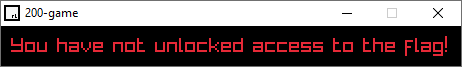
\includegraphics{200_not_unlocked}
\caption{Okienko programu z informacją o braku dostępu do flagi}
\end{figure}

Użytkownik otwiera plik wykonywalny w programie IDA\footnote{
Darmowa wersja programu IDA przeznaczona do użytku domowego dostępna do pobrania pod adresem 
\url{https://www.hex-rays.com/products/ida/support/download_freeware}},
aby zapoznać się z działaniem programu.

\begin{figure}[H]
\centering
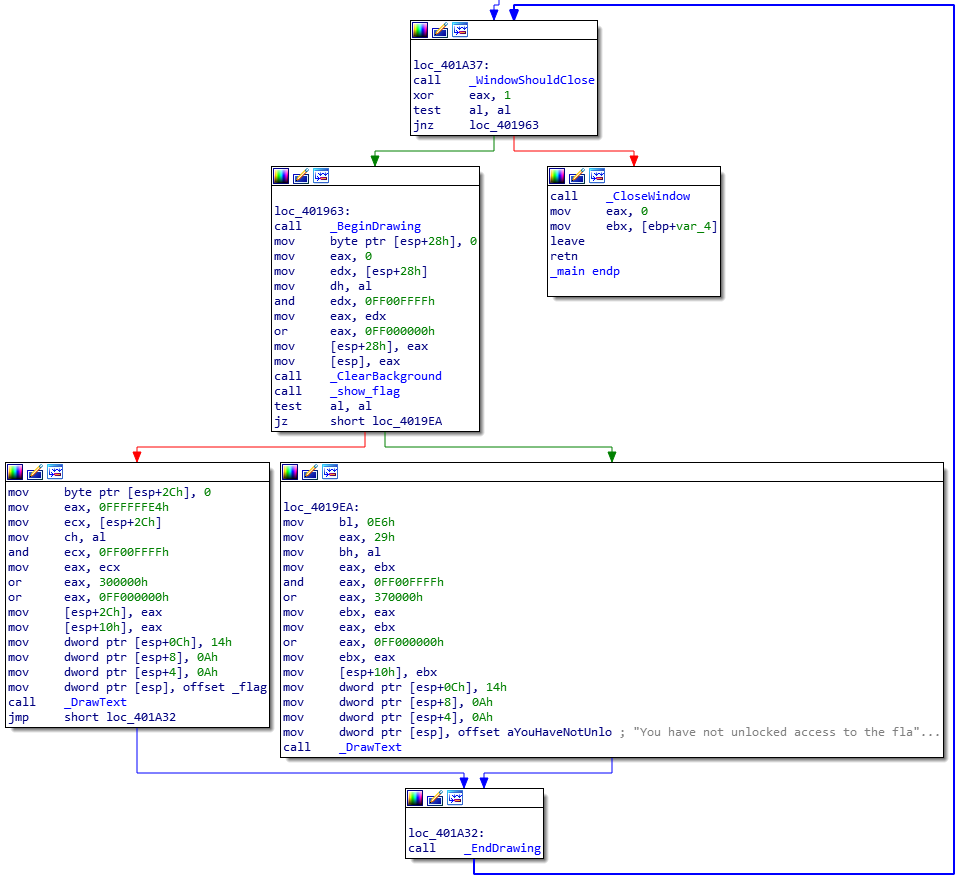
\includegraphics[width=\textwidth]{200_ida_graph}
\caption{Widok grafowy w programie IDA przestawiający główną pętle programu}
\end{figure}

Zauważa on, że wywołanie funkcji o nazwie \emph{\_show\_flag} decyduję o wyborze jednego
z dwóch węzłów wywołania programu. Biorąc pod uwagę nazwę tej funkcji oraz tekst
wyświetlany w prawym węźle (\textit{,,You have not unlocked access to the fla''...}), domyśla
się, że funkcja \emph{\_show\_flag} decyduję o tym czy flaga zostanie wyświetlona użytkownikowi.

\begin{figure}[H]
\centering
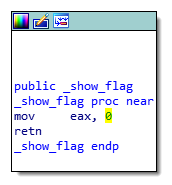
\includegraphics{200_ida_show_flag}
\caption{Kod asemblera x86 dla funkcji \emph{\_show\_flag}}
\end{figure}

Jedyne co ta funkcja robi to zwraca liczbę 0 -- czyli \emph{false}.
Próbuję on więc spatchować\footnote{Patchowanie w tym wypadku oznacza modyfikowanie programu
wykonywalnego poprzez nadpisanie konkretnych bajtów}
program, aby funkcja ta zwracała 1 -- czyli \emph{true}.

\begin{figure}[H]
\centering
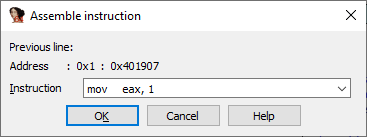
\includegraphics{200_ida_patch}
\caption{Modyfikacja instrukcji, aby zwracała 1 zamiast 0}
\end{figure}

Po zaaplikowaniu patch'a oraz ponownym uruchomieniu programu użytkownikowi ukazuję się
następujący widok.

\begin{figure}[H]
\centering
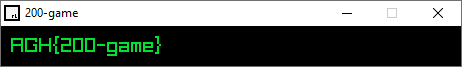
\includegraphics{200_flag}
\caption{Okienko programu wraz z otrzymaną flagą}
\end{figure}

Po wpisaniu na stronie flagi \emph{AGH\{200-game\}} użytkownik otrzymuję informację
o poprawnym rozwiązaniu zadania.

\section{Zadanie 300-strcmp}

Użytkownik pobiera plik \emph{strcmp} i sprawdza go programem \emph{file}.

\begin{minted}[breaklines]{text}
$ file strcmp
strcmp: ELF 64-bit LSB pie executable, x86-64, version 1 (SYSV), dynamically linked, interpreter /lib64/ld-linux-x86-64.so.2, BuildID[sha1]=bda67999b52d8f4d1f9456346119790c47c261d8, for GNU/Linux 3.2.0, stripped
\end{minted}

Dowiaduje się, że jest to 64-bitowy plik wykonywalny na platformę Linux.
Uruchamia więc go, aby sprawdzić jego działanie.

\begin{minted}{text}
$ ./strcmp
Enter the flag: test
Incorrect flag!
\end{minted}

Aby przeanalizować działanie programu otwiera go w darmowym narzędziu Cutter\footnote{\url{https://cutter.re/}}

\begin{figure}[H]
\centering
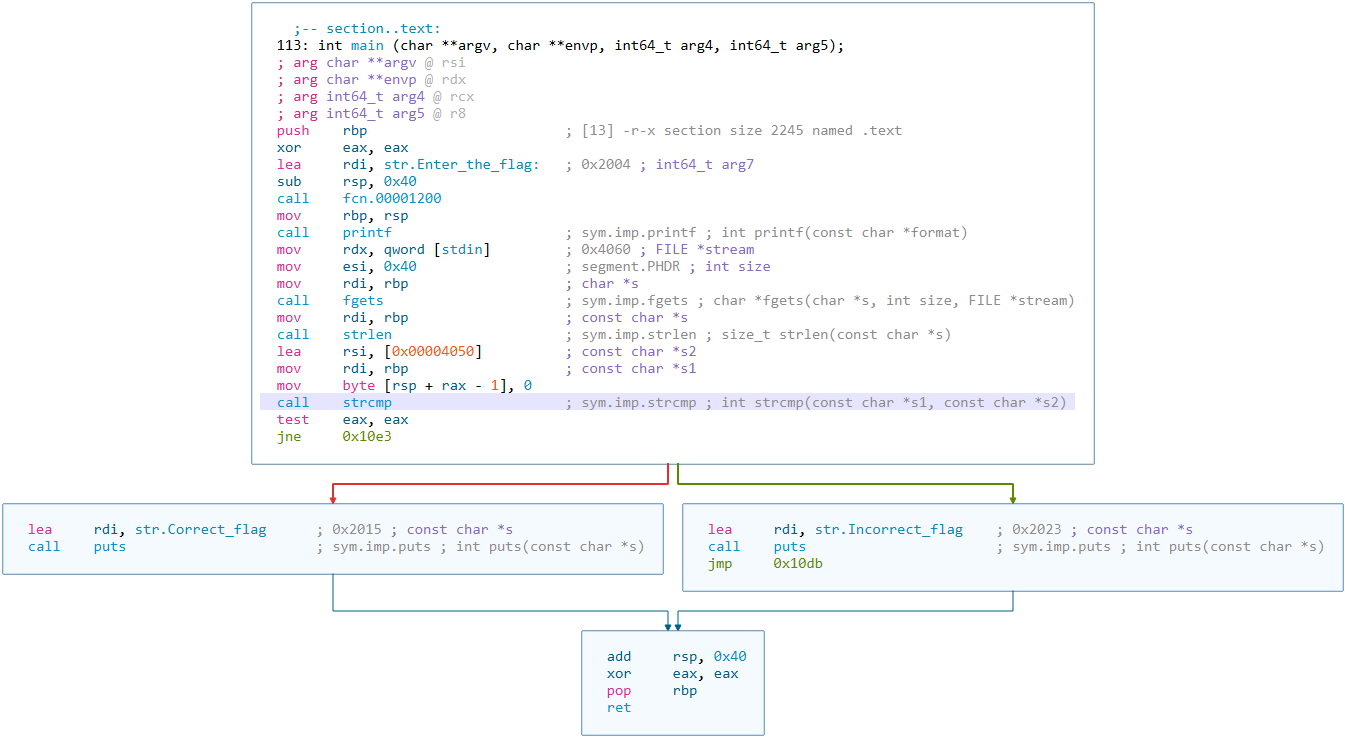
\includegraphics[width=\textwidth]{300_cutter}
\caption{Widok grafowy funkcji \emph{main} w narzędziu Cutter}
\end{figure}

Zauważa, że za sprawdzenie poprawności flagi odpowiada funkcja \emph{strcmp}, która
jako jednego z argumentów używa niemodyfikowanego wejścia użytkownika.
Oznacza to, że flaga również musi być przekazana w jawnej formie do tej funkcji.
Korzysta on więc z GNU Debugger, aby odczytać przekazany do niej drugi parametr.

\begin{minted}{text}
$ gdb -q strcmp
Reading symbols from strcmp...
(No debugging symbols found in strcmp)
(gdb) info functions strcmp
All functions matching regular expression "strcmp":

Non-debugging symbols:
0x0000000000001070  strcmp@plt
\end{minted}

Zakłada teraz punkt przerwania w momencie wywołania funkcji \emph{strcmp}.

\begin{minted}{text}
(gdb) break strcmp@plt
Breakpoint 1 at 0x1070
\end{minted}

Uruchamia program i wpisuje dowolny tekst, aby przejść do punktu przerwania.

\begin{minted}{text}
(gdb) run
Starting program: /home/piotr/strcmp 
Enter the flag: test

Breakpoint 1, 0x0000555555555070 in strcmp@plt ()
\end{minted}

Kiedy program zatrzyma się w pożądanym miejscu, użytkownik podgląda zawartość pamięci na którą
zgodnie z konwencją wywołania System V AMD64\footnote{
\url{https://en.wikipedia.org/wiki/X86_calling_conventions\#System_V_AMD64_ABI}}
wskazują rejestry RDI oraz RSI - czyli dwa parametry przekazane do funkcji \emph{strcmp}.

\begin{minted}{text}
(gdb) x/s $rdi
0x7fffffffe2b0: "test"
(gdb) x/s $rsi
0x555555558050: "AGH{300-strcmp}"
\end{minted}

W rejestrze RDI znajduję się adres tekstu wpisanego przez użytkownika, natomiast
w rejestrze RSI ciąg znaków, z którym wejście od użytkownika jest porównywane -- czyli
jawna postać flagi. W taki sposób użytkownik otrzymuję flagę \emph{AGH\{300-strcmp\}},
która jest rozwiązaniem tego zadania.

\section{Zadanie 400-decrypt}

Użytkownik pobiera plik \emph{decrypt} i podobnie jak wcześniej sprawdza go programem \emph{file}.

\begin{minted}[breaklines]{text}
$ file decrypt
decrypt: ELF 64-bit LSB pie executable, x86-64, version 1 (SYSV), dynamically linked, interpreter /lib64/ld-linux-x86-64.so.2, BuildID[sha1]=8b4924f98f391fb9939f323d9a89e37d2e7febb7, for GNU/Linux 3.2.0, not stripped
\end{minted}

Podobnie jak w poprzednim zadaniu, dowiaduję się, że jest to 64-bitowy linuksowy program.
Uruchamia go.

\begin{minted}{text}
$ ./decrypt
Enter the flag: test
Incorrect flag!
\end{minted}

Tym razem do analizy programu użyje narzędzia Ghidra\footnote{\url{https://ghidra-sre.org/}}.
Potrafi ona zamieniać kod maszynowy programu na psuedokod C, co bardzo ułatwia
analizowanie plików wykonywalnych.
Użytkownik wczytuje pobrany plik wykonywalny do narzędzia i uruchamia widok dekompilatora
dla funkcji \emph{main}.

\begin{figure}[H]
\centering
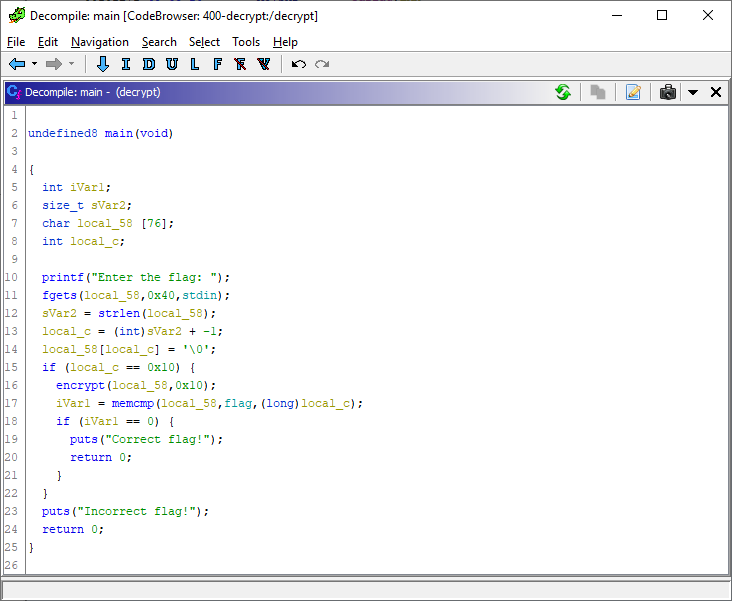
\includegraphics[width=\textwidth]{400_main}
\caption{Widok dekompilatora dla funkcji \emph{main} w narzędziu Ghidra}
\end{figure}

Zauważa, że powyższy fragment kodu szyfruje tekst wprowadzony przez użytkownika,
a następnie porównuje go z ciągiem znaków zawartym w zmiennej \emph{flag}.
Następnie analizuje zdekompillwany kod funkcji \emph{encrypt} zmieniając nazwy zmiennych
dla poprawy czytelności.

\begin{figure}[H]
\centering
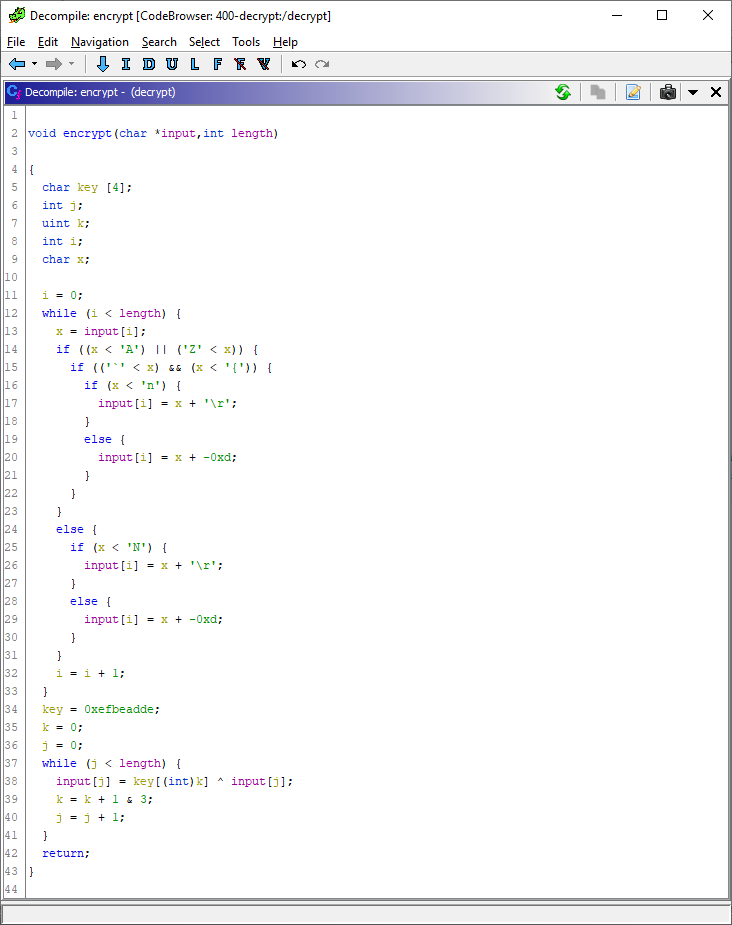
\includegraphics[width=\textwidth]{400_encrypt}
\caption{Widok dekompilatora dla funkcji \emph{encrypt} w narzędziu Ghidra}
\end{figure}

Zauważa, że funkcja szyfrująca dzieli się na dwa fragmenty.
Pierwszy fragment przechodzi po każdym znaku tablicy wejściowej i dodaje
\emph{'\textbackslash r'} lub
odejmuje \emph{0xd} w zależności czy dany znak spełnia warunki.
Zarówno \emph{'\textbackslash r'} jak i \emph{0xd} to 13 w systemie dziesiętnym.
Analizując warunki dochodzi do wniosku, że jest to prosty szyfr przesuwający zwany ROT13.
Drugi fragment również przechodzi po każdym znaku tablicy, a następnie wykonuje
operacje XOR z kolejnymi bajtami klucza. Po przekroczeniu ostatniego bajtu klucza
wraca do pierwszego, co zapewnia operacja \mintinline{c}{k = k + 1 & 3}.
Biorąc pod uwagę, że liczby całkowite przechowywane
są w pamięci w formie Little Endian, to klucz również można zapisać następująco:
\emph{0xDE, 0xAD, 0xBE, 0xEF}. Następnie podgląda zawartość tablicy \emph{flag}.

\begin{figure}[H]
\centering
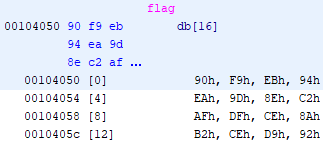
\includegraphics{400_flag}
\caption{Zawartość tablicy \emph{flag} w widoku Listing narzędzia Ghidra}
\end{figure}

Posiadając te informacje pisze skrypt w języku Python, który odwróci wcześniej otrzymaną
tablice \emph{flag} do wartości pierwotnej.

\begin{minted}[breaklines]{python}
flag = [0x90, 0xF9, 0xEB, 0x94, 0xEA, 0x9D, 0x8E, 0xC2, 0xAF, 0xDF, 0xCE, 0x8A, 0xB2, 0xCE, 0xD9, 0x92]

key = [0xDE, 0xAD, 0xBE, 0xEF]
for i in range(len(flag)):
    flag[i] ^= key[i % len(key)]

for i in range(len(flag)):
    c = flag[i]

    if c >= ord("A") and c <= ord("Z"):
        if c + 13 <= ord("Z"):
            flag[i] = c + 13
        else:
            flag[i] = c - 13
    elif c >= ord("a") and c <= ord("z"):
        if c + 13 <= ord("z"):
            flag[i] = c + 13
        else:
            flag[i] = c - 13

print("".join([chr(x) for x in flag]))
\end{minted}

Zapisuje skrypt jako \emph{decrypt.py} i uruchamia go.

\begin{minted}{text}
$ python decrypt.py
AGH{400-decrypt}
\end{minted}

Otrzymuje rozwiązanie tego zadania, czyli flagę \emph{AGH\{400-decrypt\}}.

\section{Zadanie 500-secret-shell}

W tym zadaniu zamiast pliku do pobrania, użytkownik otrzymuje następującą informację:

\begin{minted}{text}
$ ssh ctf@szczygiel.dev -p 2222
ctf@szczygiel.dev's password: agh-reverse-engineering
\end{minted}

Uruchamia więc terminal i zgodnie ze wskazówkami loguje się na zadany host.
W katalogu \emph{/home/admin/} znajduje następujące pliki:

\begin{minted}{text}
ctf@d35da2ee92fe:/home/admin$ ls -l
total 20
-rw------- 1 admin admin    22 Dec 11 21:26 access_code.txt
-rwsr-xr-x 1 admin admin 16332 Dec 11 21:26 secret-shell
\end{minted}

Zauważa plik \emph{access\_code.txt}, w którym prawdopodobnie znajduję się flaga.
Niestety użytkownik \emph{ctf} nie posiada uprawnień do odczytania tego pliku.
Jest też plik wykonywalny z ustawionym bitem SUID\footnote{
\url{https://en.wikipedia.org/wiki/Setuid\#When_set_on_an_executable_file}}.
Oznacza to, że można uruchomić program \emph{secret-shell} z prawami użytkownika \emph{admin}.
Uruchamia więc program \emph{secret-shell}.

\begin{minted}{text}
ctf@d35da2ee92fe:/home/admin$ ./secret-shell
Welcome, enter your name: Piotr
Hello, Piotr

Enter the access code: test
Access denied!
\end{minted}

Pobiera ten program na lokalny komputer w celu jego przeanalizowania.

\begin{minted}{text}
$ scp -P 2222 ctf@szczygiel.dev:/home/admin/secret-shell .
\end{minted}

Analizuje go narzędziem Ghidra. Rzuca mu się w oczy funkcja \emph{greeter} w której
imie użytkownika pobierane jest niebezpieczną funkcją \emph{gets}. Jest ona niebezpieczna,
ponieważ nie kontroluje ona długości pobieranego wejścia i może prowadzić do przepełnienia
bufora \emph{name} o rozmiarze 72 bajtów.

\begin{figure}[H]
\centering
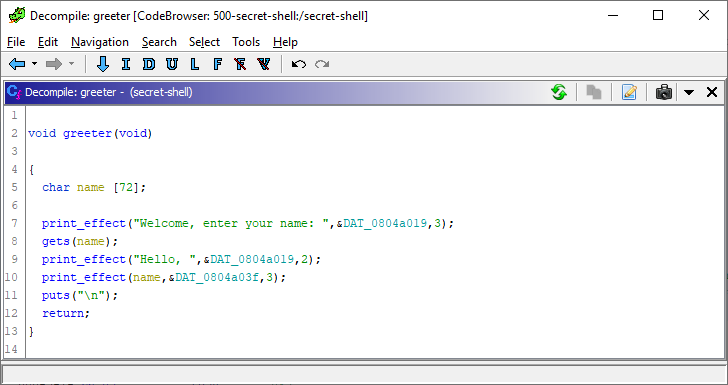
\includegraphics[width=\textwidth]{500_greeter}
\caption{Widok dekompilatora dla funkcji \emph{greeter} w narzędziu Ghidra}
\end{figure}

Znajduję również funkcję \emph{access\_secret\_shell}, która uruchamia powłokę systemową.
Pamiętając o ustawionym bicie SUID, oznacza to, że uruchomiona powłoka będzie z uprawnieniami
użytkownika \emph{admin}.

\begin{figure}[H]
\centering
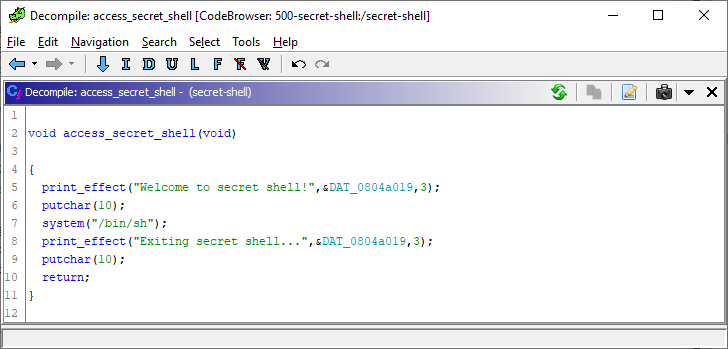
\includegraphics[width=\textwidth]{500_access}
\caption{Widok dekompilatora dla funkcji \emph{access\_secret\_shell} w narzędziu Ghidra}
\end{figure}

Sprawdza zabezpieczenia programu wykonywalnego skryptem \mintinline{text}{checksec.sh}\footnote{
\url{https://github.com/slimm609/checksec.sh}} i dowiaduje się, że wyłączony jest Stack Canary\footnote{
\url{https://en.wikipedia.org/wiki/Buffer_overflow_protection\#Canaries}} oraz że plik nie jest
position-independent executable\footnote{\url{https://en.wikipedia.org/wiki/Position-independent_code}}.
Dochodzi więc do wniosku, że będzie mógł on wykonać atak Stack buffer overflow\footnote{
\url{https://en.wikipedia.org/wiki/Stack_buffer_overflow}} nadpisujący adres powrotu
z funkcji \emph{greeter}.

Odpowiednio przepełniając bufor \emph{name}, będzie on mógł nadpisać adres powrotu
funkcji. Dzięki temu po wyjściu z funkcji \emph{greeter} program przeniesie się do
wskazanego przez niego miejsca.

\begin{figure}[H]
\centering
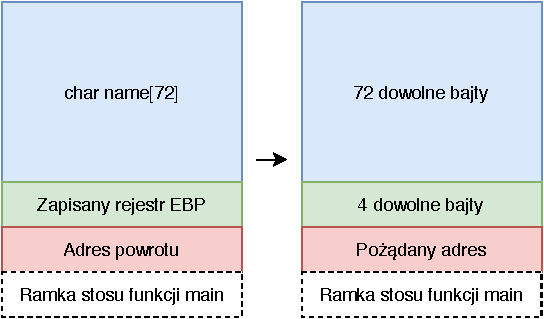
\includegraphics[width=\textwidth]{500_stack}
\caption{Zawartość stosu funkcji \emph{greeter} przed i po ataku}
\end{figure}

Aby rozwiązać zadanie, będzie potrzebował znaleźć takie miejsce w programie, gdzie
po przeniesieniu się do niego uzyska w jakiś sposób dostęp do pliku \emph{access\_code.txt}.
Idealnym do tego miejscem jest funkcja \emph{access\_secret\_shell}.

\begin{figure}[H]
\centering
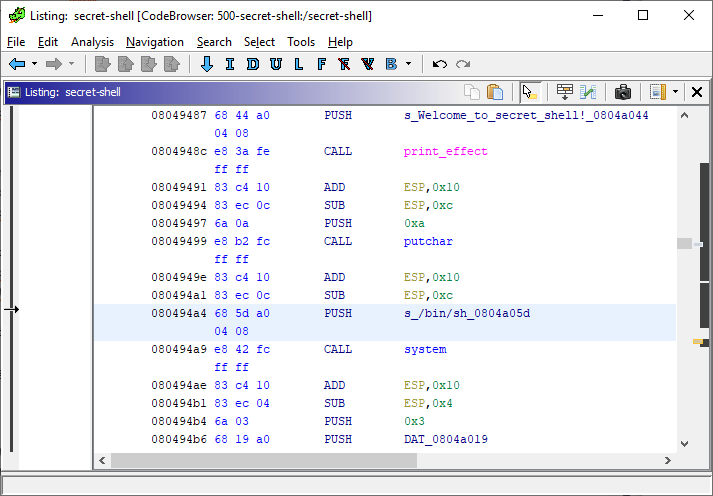
\includegraphics[width=\textwidth]{500_bin_sh_address}
\caption{Fragment funkcji \emph{access\_secret\_shell} uruchamiający powłokę}
\end{figure}

Wybrany przez niego adres to \emph{080494a4} -- kiedy wykonanie programu przeniesie się w to miejsce,
na stos zostanie wrzucony wskaźnik do ciągu \emph{/bin/sh}, a następnie zostanie wywołana
funkcja \emph{system}, tym samym uruchamiając powłokę systemową. Wtedy korzystając z poleceń
powłoki będzie mógł wyświetlić zawartość pliku \emph{access\_code.txt}.

Pozostaje mu więc tylko przygotować exploit, który przepełni bufor
w taki sposób, aby adres powrotu wskazywał właśnie na to miejsce. Musi też pamiętać
o tym, że adresy w pamięci przechowywane są w formacie Little Endian, więc adres
\emph{080494a4} będzie musiał przekazać jako \emph{a4940408}.

Przygotowuje więc prosty jednolinijkowiec w języku Python 2, wypisujący ciąg znaków,
który wypełni bufor oraz zapisany rejestr EBP literkami \emph{A},
a następnie doda pożądany adres:

\mintinline{python}{print 'A' * 76 + '\xa4\x94\x04\x08'}

\begin{figure}[H]
\centering
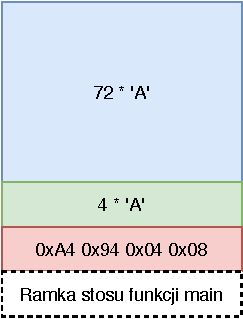
\includegraphics[width=6cm]{500_overflow}
\caption{Zawartość stosu funkcji \emph{greeter} po wykonaniu exploita}
\end{figure}

Pozostało mu już tylko wykonać exploit na zdalnej maszynie. Jednak samo przekazanie
wyjścia tego skryptu na wejście programu \emph{secret-shell} nie zadziała, ponieważ
po przekazaniu pożądanego ciągu znaków zamknie się standardowe wejście.
Z tego powodu powłoka \emph{/bin/sh} natychmiast się wyłączy.

Korzysta on więc z prostego triku, który po wywołaniu programu zachowuje dostęp
do standardowego wejścia, dzięki programowi \mintinline{text}{cat}.

\begin{minted}[breaklines]{text}
ctf@de4848f994a7:/home/admin$ (python2 -c "print 'A' * 76 + '\xa4\x94\x04\x08'"; cat) | ./secret-shell
\end{minted}

\begin{figure}[H]
\centering
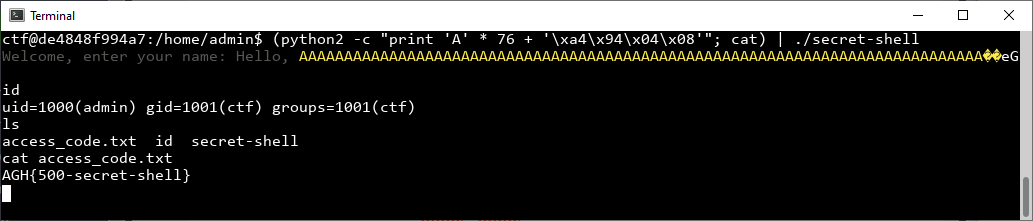
\includegraphics[width=\textwidth]{500_solution}
\caption{Uruchomienie exploita i rozwiązanie zadania}
\end{figure}

W taki sposób otrzymuje rozwiązanie zadania, czyli flagę \emph{AGH\{500-secret-shell\}}.

\section{Zadanie 600-vm}

\backmatter

\cleardoublepage
\listoffigures

%\cleardoublepage
%\listoftables

\cleardoublepage
\printbibliography

\end{document}
